%%%%%%%%%%%%%%%%%%%%% chapter.tex %%%%%%%%%%%%%%%%%%%%%%%%%%%%%%%%%
%
% sample chapter
%
% Use this file as a template for your own input.
%
%%%%%%%%%%%%%%%%%%%%%%%% Springer-Verlag %%%%%%%%%%%%%%%%%%%%%%%%%%

\chapter{Reti Neurali Artificiali}
In questo caso oltre alla classificazione parliamo anche di previsione, per esempio dato un valore l'obiettivo è quello di stimare il valore in uscita(regressione lineare).  L'adaline è un modello lineare quindi ci porterà a progettare un sistema di classificazione lineare, come ben sappiamo il limite di un modello lineare è quello che si appresta a classificare bene soltanto dati linearmente separabili, purtroppo non è sempre così e devono essere introdotte superfici di decisione più complesse. 

\section{Introduzione}
Le reti neurali possono essere spiegate dal punto di vista ingegneristico (progettazione di sistemi), ma possono anche essere spiegate descrivendo cos'è un neurone, quindi da un punto di vista cibernetico. Un neurone trasmette segnali elettrici ai neuroni che si trovano nel suo vicinato utilizzando dei filamenti, e questi segnali elettrici sono fondamentalmente neurotrasmettitori. Il problema da risolvere è questo: è possibile con questi modelli così elementari, agglomerati in qualche modo in una struttura o topologia complessa, a fornire una superficie di decisione che non sia sempre un iperpiano laddove l'iperpiano non è sufficiente?
\begin{figure}
\centering
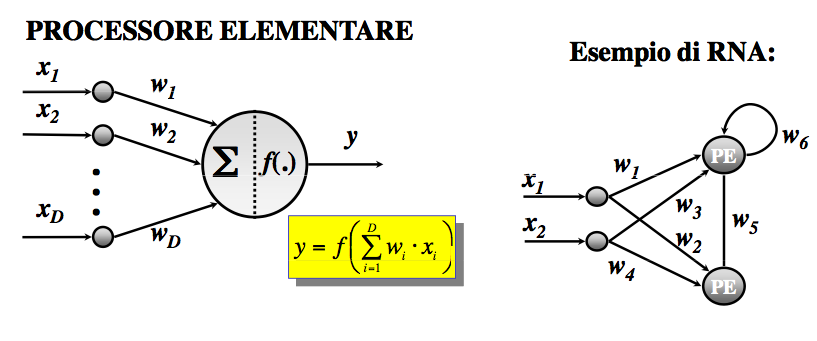
\includegraphics[scale=0.5]{img/rete_neurale.png}
\label{reti}
\end{figure}
\noindent In figura \ref{reti} rivediamo il sistema adattativo, ma in questo caso i neuroni non sono tutti dello stesso tipo, alcuni sono soltanto recettivi mentre altri sono elementi di elaborazione, inoltre ci sono anche quelli che producono il risultato. Gli $x_i$ (che sono gli input) sono associati a dei neuroni che semplicemente catturano l'input e passano l'input, quindi non lo trasformano, mentre il nodo elaborativo (PE) lo possiamo associare a quello che ne fa un elaborazione. L'arco uscente dal neurone input e giunge al neurone output (PE) è pesato da $w_i$, quindi il neurone elaborativo (PE) non fa altro che la sommatoria del prodotto dell'input corrispondente con il peso associato all'arco entrante. Questa è detta funzione di attivazione  e la indichiamo genericamente con $f$, nel caso dell'adaline è una funzione lineare quindi la sommatoria del prodotto dei valori di input con i pesi delle connessioni incidenti. Ma posso anche prevedere una funzione non lineare, quindi una funzione qualsiasi. Il neurone che abbiamo descritto è uno dei tanti neuroni che possono entrare in gioco nella nostra struttura neurale più complessa. La rete neurale artificiale può essere vista come un grafo dove ci sono dei nodi alcuni dei quali sono esclusivamente di input, altri dei quali sono di output, e la cosa particolare è che almeno per il momento non ci sono connessioni che vanno dal neurone output al neurone input, ma ci sono soltanto connessioni che vanno dal neurone di input al neurone di output. \'E possibile in questo caso che il neurone output possa essere di input a se stesso.\\

\noindent I parametri che entrano in gioco sono la topologia, il numero di vertici, il numero degli archi, i pesi degli archi e la funzione $f$.\\

\noindent McCalloch e Pitts nel 43' hanno già progettato il modello in figura \ref{pemc} che prende il nome proprio dai sui ideatori.
\begin{figure}
\centering
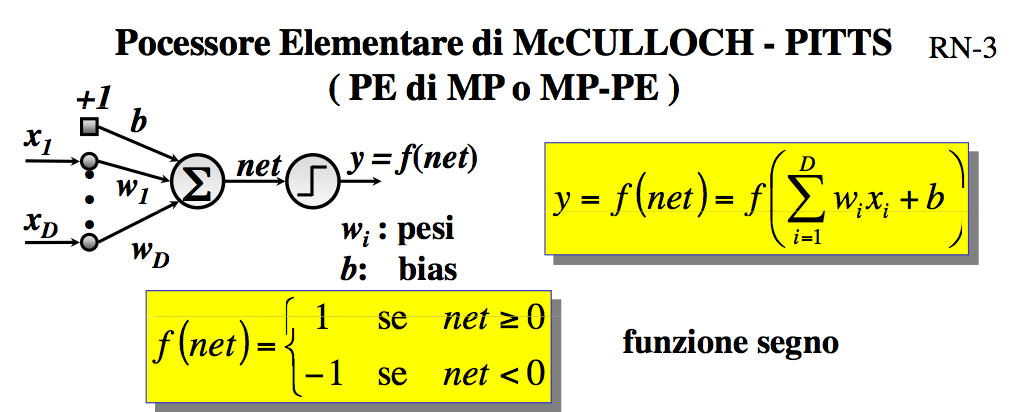
\includegraphics[scale=0.5]{img/PEMC.png}
\caption{Processore elementare di McCalloch e Pitts }
\label{pemc}
\end{figure}
Il processore opera in questo modo:  ci sono $d$ neuroni in input ed il neurone $b$ di \emph{bias}, si effettua la sommatoria ma questa volta la funzione è una funzione a gradino, quindi 
\begin{equation}
y=f(net) = f \left( \sum_{i=1}^d w_i x_i +b\right)
\end{equation}
e la $f(net)$ può assumere valore $1$ se l'argomento è $\geq 0$ o $-1$ se l'argomento è $< 0$
\[
f(net)=
\begin{cases}
1 & \text{se} \ net \geq 0\\
-1 & \text{se} \ net < 0 
\end{cases} 
\]
\noindent Questo modello ha una serie di proprietà
\begin{itemize}
\item Può separare solo due classi
\item La funzione discriminante è un iperpiano nello spazio a $d$ dimensioni di equazione : $w_1 x_1 + w_2 x_2 + \dots + w_d x_d + b = 0$. $b$  nel caso di una retta è l'intercetta, invece nel caso di un iperpiano è la distanza dall'origine.
\item la funzione soglia divide lo spazio in due semi-spazi a cui attribuisce tutti i pattern per cui la funzione assume valori +1 e dall'altra parte tutti i pattern che la funzione assume  -1.
\end{itemize}
Il sistema si può applicare al caso multiclasse utilizzando la tecnica \emph{one-versus-one} oppure $\emph{one-live-out}$.\\

\noindent La sudduvisione netta appena vista è troppo hard, allora introduciamo un po' \emph{soft computing}, introduciamo un po' di smussatura nella transizione dal passaggio di pattern che appartengono ad una classe e pattern che appartengono ad un altra classe.  Quindi la superficie di decisione non è un iperpiano ma è una superficie di decisione generica. Una funzione che si comporta in questo modo potrebbe essere la funzione tangente iperbolica (Figura \ref{funzioni}) che per come è strutturata ci consente di passare da -1 a 1.
\begin{figure}
\centering
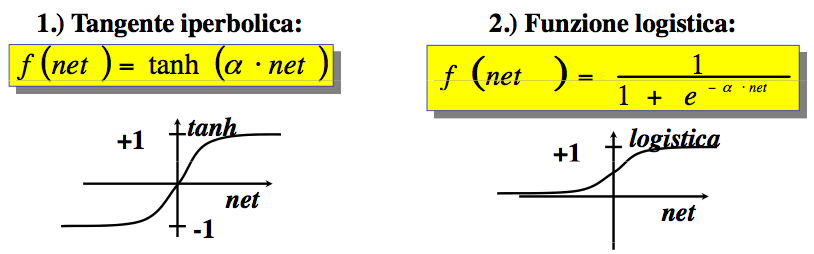
\includegraphics[scale=0.6]{img/funzioni.png}
\caption{Funzioni}
\label{funzioni}
\end{figure}
Nella figura \ref{funzioni} $\alpha$ è un fattore di intensificazione dell'argomento. Lo stesso vale anche per la funzione logistica, questa volta il passaggio è da 0 a 1. In entrambi i casi sono funzioni asintotiche  agli estremi, quindi non assumeranno mai il valore -1 o 1 nel caso della tangente iperbolica, oppure 0 o 1 per la funzione logistica. Quindi
\begin{itemize}
\item Reti Neurali Artificiali con funzioni a soglia creano superfici di decisione lineari a tratti
\item Reti Neurali Artificiali con funzioni sigmoidali creano superfici di decisione molto complesse e non-lineari
\end{itemize}

\section{Learning Supervisionato}
IL PE-MP non aveva apprendimento, non aveva la capacità di modificare i parametri, l'idea loro era quella di realizzare sistemi che fossero cablati per il problema, cioè i pesi venivano determinati a mano, in modo tale che funzionasse il sistema per un certo problema specifico, quindi non c'era l'idea di fornire della coppie di ingresso e di uscita desiderata in modo tale da avere un apprendimento dei parametri in modo automatico. 

\subsection{Perceptron Algorithm}
Rosemblatt introduce l'apprendimento per il PE-MP con un algoritmo di addestramento che prende il nome di percettrone. 
\begin{description}
\item[Step 1] Si presenta un campione $x \in C_1$
\item[Step 2] Se l'uscita è corretta allora non fare nulla. Nota: il modello produce o 1 o -1 quindi già sappiamo che l'output è uno di questi due valori. Quindi se produce l'output corretto l'errore è 0 altrimenti l'errore è 2.
\item[Step 3] Se invece l'uscita non è corretta allora modifica i pesi ed il bias finché l' uscita è corretta
\item[Step 4] Ripetere l’operazione finché tutti i pattern non siano correttamente classificati 
\end{description}
Se l'errore complessivo su tutte le coppie input output desiderato lo misuro sempre con MSE allora la regola di aggiornamento dei paesi è
\begin{equation}
w(n+1) = w(n)+\eta \cdot(d(\eta) - y(\eta)) \cdot x(\eta)
\end{equation}
in sinstesi modifico i pesi in modo tale da aggiungere il pattern al peso, cioè incremento il peso attuale utilizzando il pattern in ingresso. L' algoritmo di Rosemblatt è esattamente l'adaline nel caso in cui $\eta=0.5$ e nel caso in cui la funzione di attivazione è la funzione segno.\\
\noindent Il modello di MP impara soltanto quando l'uscita è errata. Quindi il modello di MP con l'algoritmo di rosemblatt è un modello che
\begin{itemize}
\item Classifica due classi
\item si comporta correttamente quando l'uscita è corretta e apprende quando l'uscita non è corretta
\item La superficie di decisione è lineare, quindi un iperpiano.
\end{itemize}
Facendo apprendimento passo dopo passo se si va a modificare i pesi per apprendere la coppia corrente non è garantito che non vengano variate le prestazioni per le coppie precedenti. \\

\noindent Per espandere al modello non lineare allora è necessario creare reti di neuroni. Quindi una gerarchia formata da neuroni di input, altri strati di neuroni ed infine i neuroni di output. Gli strati di neuroni interni vengono detti neuroni hidden.

\subsection{Regola a catena}
La regola a catena ci consente di affrontare il problema dell'apprendimento in modo abbastanza semplificato,  apprendere dei pesi equivale a determinare i valori dei parametri rispetto ad un criterio di soddisfacimento. Questo criterio di soddisfacimento è la funzione di errore che si commette nel misurare lo scostamento che intercorre tra il valore calcolato dal neurone ed quello che invece dovrebbe effettivamente produrre, che è il target desiderato. Per fare questo misuriamo gli errori dello stesso neurone su tutti quanti i campioni, ovviamente nel caso di una rete di neuroni, questo procedimento viene effettuato su tutti i neuroni e quindi non è altro che una doppia sommatoria.  Dato un dataset di training di $n$ campioni, dove ogni campione è un pattern $p_i = [x_1, x_2, \dots, x_p]$, dato il valore desiderato $d_p$, l'obiettivo è quello di calcolare i pesi $w$ minimizzando lo scostamento tra il valore desiderato e l'output restituito. Nel caso più semplice abbiamo un solo input, quindi  $y_p = w x_p$, in questo caso banale in cui abbiamo un solo peso dobbiamo derivare la funzione $J$ rispetto a $w$ e porla uguale a zero, per poi calcolare il valore di $w$ per il quale si minimizza la funzione costo $J$.
\begin{equation}
J = \frac{1}{2} \sum_p (d_p - y_p)^2 = \sum_p J_p
\end{equation}
dove $J_p$ è la funzione costo del $p$-esimo campione ed $y_p = w x_p$. Quindi calcoliamo la derivata parziale di $J$ rispetto a $w$ ($\frac{\partial J_p}{\partial w}$). Questa derivata la possiamo scomporre in virtù di una regola di derivazione di funzioni composte che dice sia $y=f(x)$ con $f$ differenziabiile allora
\begin{equation}
\frac{\partial y}{\partial x} = \frac{\partial y}{\partial f} \cdot \frac{\partial f}{\partial x} 
\end{equation}
questa banale regola di derivazione la si può applicare anche nel caso di $J$ quindi
\begin{equation}\label{184}
\frac{\partial J_p}{\partial w} = \frac{\partial J_p}{\partial y_p} \cdot \frac{\partial y_p}{\partial w}
\end{equation}
calcoliamo la $\frac{\partial J_p}{\partial y_p}$
\begin{equation}
\frac{\partial J_p}{\partial y_p} = 2(d_p - y_p) \cdot der(-y_p) \cdot \frac{1}{2} = 2(d_p - y_p) \cdot -1 \cdot \frac{1}{2} = -(d_p - y_p) 
\end{equation}
calcoliamo poi $\frac{\partial y_p}{\partial w}$ che è facile perchè essendo $y_p = w x_p$ allora la derivata è esattamente $x_p$, qundi
\begin{equation}
\frac{\partial J_p}{\partial w} = \frac{\partial J_p}{\partial y_p} \cdot \frac{\partial y_p}{\partial w} = -(d_p - y_p) \cdot x_p = -\varepsilon_p x_p
\end{equation}
La regola del gradiente discendente dice che il valore di $w$ viene incrementato di una quantità che è direttamente proporzionale a $-\eta \nabla J(k)$
\begin{equation}
w(k+1) = w(k) - \eta \nabla J(k)
\end{equation}
quindi indipendentemente da $\eta$ il gradiente di $J$ rispetto a $w$ al passo $k$ va calcolato semplicemente come abbiamo visto sopra, ovvero la derivata parziale $\frac{\partial J_p}{\partial w}$. Quindi andando a sostituire abbiamo
\begin{equation}
w(k+1) = w(k) + \eta \  \varepsilon_n x_n 
\end{equation}
possiamo affermare che l'incremento è direttamente proporzionale all'errore commesso, cioè allo scostamento ottenuto moltiplicato per l'input. \\

\noindent Adesso vediamo come cambia la regola di apprendimento nel caso di funzioni non lineari. Questa volta non abbiamo più la semplice combinazione lineare $y_p= \sum w x_p$ ma abbiamo una funzione di questa combinazione lineare (tipicamente viene attribuito il nome \emph{net} alla sommatoria) quindi abbiamo $y=f(net)$ dove $f$ è la funzione di attivazione (che come abbiamo visto può essere la funzione tangente iperbolica, la funzione logistica, quindi funzioni continue non lineari).  Vediamo adesso cosa succede nel caso di funzioni non lineari. Applichiamo la regola di derivazione come fatto in precendenza. Questa volta la derivata di $\frac{\partial y_p}{\partial w}$ può essere scritta come 
\begin{equation}
\frac{\partial y_p}{\partial w_i} = \frac{\partial y_p}{\partial net_p} \cdot \frac{\partial net_p}{\partial w_i} 
\end{equation}
ricordiamo che la funzione costo è
\begin{equation}
J = \frac{1}{2N} \sum_{p=1}^N (d_p - y_p)^2
\end{equation}
dove $p$ è l'indice di pattern, e
\begin{equation}
y_p = f \left( \sum_i w_i \cdot x_{ip} \right)
\end{equation}
dove $i$ è l'indice di peso. Quindi andando a sostituire $\frac{\partial y_p}{\partial w_i}$ nella \ref{184} abbiamo
\begin{equation}
\frac{\partial J_p}{\partial w} = \frac{\partial J_p}{\partial y_p} \cdot \frac{\partial y_p}{\partial net_p} \cdot \frac{\partial net_p}{\partial w_i} 
\end{equation}
la  $\frac{\partial J_p}{\partial y_p}$ è $-(d_p - y_p)$, la $\frac{\partial y_p}{\partial net_p}$ è la derivata prima di $f$ rispetto a $net_p$, mentre la derivata di $net_p$ rispetto a $w_i$ è la derivata di una sommatoria su tutti gli $i$ rispetto ad un $w_i$ specifico, quindi per tutti i $j\neq i$ la derivata parziale si annulla, invece sarà diversa da 0 soltanto per $j=i$ , mettendo insieme i tre risultati abbiamo
\begin{equation}
\frac{\partial J_p}{\partial w} = -(d_p - y_p) \cdot f'(net) \cdot x_{ip}
\end{equation}
e di conseguenza andando a sostituire nella regola del gradiente discendente otteniamo
\begin{equation}
w_i(n+1) = w_i(n) + \eta \cdot \varepsilon_p (n) \cdot f'(net_p(n)) \cdot x_{ip}(n) 
\end{equation}
quindi la non linearità di $f$ entra in gioco soltanto nel calcolo della derivata prima di $f$ rispetto a $net_p$.  Ricordiamo che la funzione $f$ è una funzione di un unica variabile, quindi per questo viene effettuata la derivata prima e non la derivata parziale. Questa regola è nota come regola delta.\\

\section{Percettrone}
\noindent Il percettrone (Fig. \ref{percet}) è un neurone specifico un pò più complesso, naturalmente ha delle sue capacità discriminatorie. Il percettrone non funziona nel caso specifico dello xor. Supponiamo un caso di classificazione dicotomico (classificazione di due classi), possiamo effettuare la classificazione in vari modi, per esempio si può utilizzare un solo neurone che discrimina 1 o -1 a seconda della classe di appartenenza. Nel caso in cui abbiamo due neuroni allora abbiamo due valori di uscita $y_1$ ed $y_2$ ed in base alla configurazione di output vince una o l'altra classe. Un esempio di codifica che si può dare è quella di attribuire una valore unitario alla classe vincente e tutti gli altri zero, quindi bisogna far si che i pesi siano tali da far vincere soltanto il neurone corrispondente alla classe a cui esso appartiene. Gli altri invece devono essere tali da far si che il valore della funzione sia sempre zero.
\begin{figure}
\centering
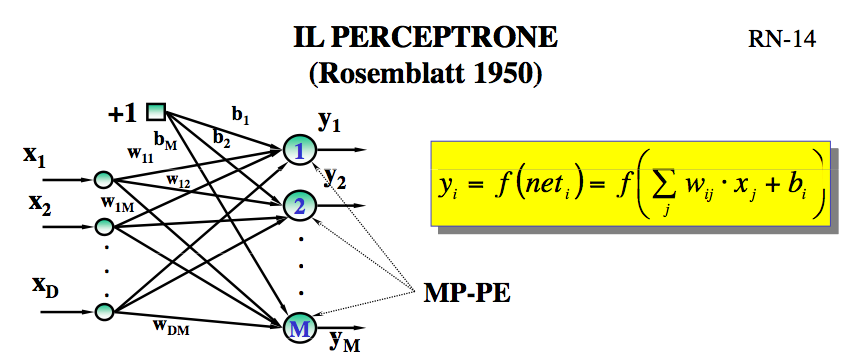
\includegraphics[scale=0.6]{img/percettrone.png}
\caption{Percettrone}
\label{percet}
\end{figure}
Si potrebbero anche codificare l'output come il sistema di numerazione binario, ma risulta molto più complicato allora e tipicamente viene utilizzata la codifica one-leave-out.  Quindi (fig \ref{percet}) se introduciamo $M$ neuroni di output vuol dire che stiamo affrontando un problema ad $M$ classi. Anche in questo caso la classificazione va bene soltanto per dati linearmente separabili, quindi li problema dello xor non è stato risolto. Anche in questo caso, come in SVM,  la superficie di decisione non è un piano qualsiasi ma sia l'iperpiano ottimo, ovvero che si mette esattamente in mezzo ai due vettori di supporto(come in SVM). 

\section{Multilayer Perceptron}
\noindent Abbiamo visto che uno dei problemi del percettrone è il problema dello xor. Per risolvere il problema viene progettata un rete denominata \emph{Multilayer Perceptron} (Fig \ref{mp}).
\begin{figure}
\centering
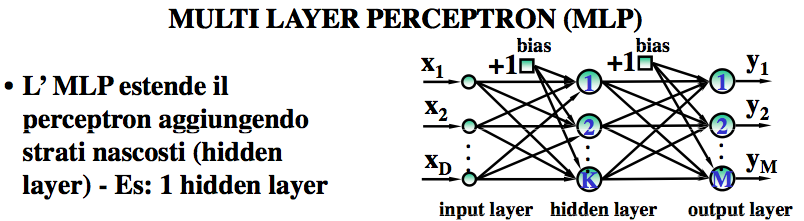
\includegraphics[scale=0.6]{img/mp.png}
\caption{Multilayer Perceptron}
\label{mp}
\end{figure}
Il problema dello xor si fonda su fatto che una retta non riesce a separare questi punti (Fig \ref{xor}),
\begin{figure}
\centering
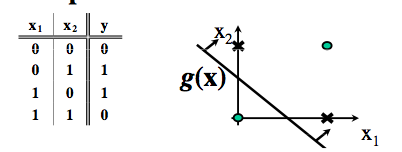
\includegraphics[scale=0.6]{img/xor.png}
\caption{Problema dello xor}
\label{xor}
\end{figure}
Quindi se ogni retta è generata da un percettrone, allora a questo punto  è necessario utilizzare due percettroni per poter avere due rette. Due percettroni raccolgono informazioni che provengono dall'input, questa combinazione la fa proprio lo strato di neuroni hidden (Fig. \ref{mp}), cioè lo strato di neuroni nascosti. Quello che osserviamo è una struttura full, cioè un grafo pienamente connesso per cui ogni neurone di input è connesso a tutti i neuroni dello strato hidden ed ogni neurone dello strato hidden è connesso a tutti i neuroni dello strato di output. Non è detto che questa rete full connessa risolve il problema, anzi di potrebbe avere un peggioramento del risultato anziché un miglioramento. Quindi alcune connessioni vanno tagliate, per scoprire quelle che vanno tagliate o ci si affida all'esperienza di chi progetta la rete oppure si fa l'apprendimento su tutta la struttura e poi durante l'apprendimento si scoprono le connessioni che peggiorano le cose. \\

\noindent In figura \ref{xor1} possiamo osservare il classico problema dello xor,  
\begin{figure}
\centering
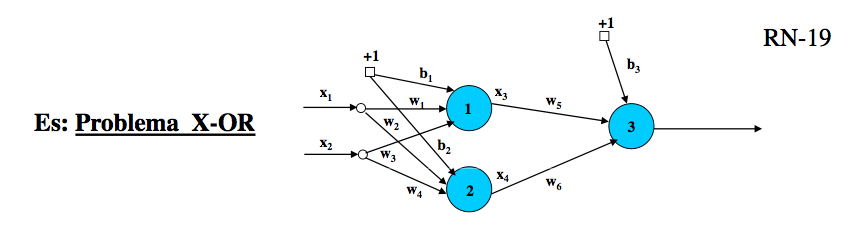
\includegraphics[scale=0.5]{img/xor1.png}
\caption{Problema xor}
\label{xor1}
\end{figure}
questa è una rete che risolve il problema. Il primo è un neurone che genera una superficie di decisione (una retta), l'altro neurone invece genera l'altra retta. Adesso però ci vuole un neurone che capisca quale  quando deve essere attivata una e quando deve essere attivata l'altra, cioè quando un pattern è all'interno delle due rette e quando è all'esterno delle due rette (Fig. \ref{xor2}), quindi 
\begin{figure}
\centering
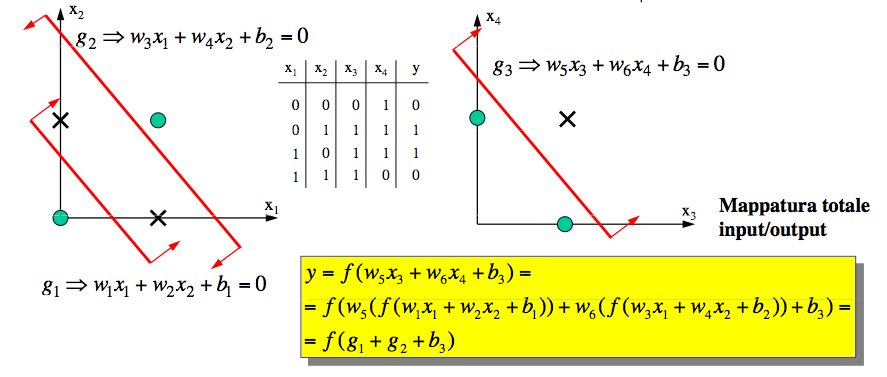
\includegraphics[scale=0.5]{img/xor2.png}
\label{xor2}
\end{figure}
i due neuroni hidden sono percettroni per determinare funzioni di decisioni lineari, l'altra invece è una funzione che governa. Se analizziamo questo sistema ci accorgiamo che conosciamo gli input ed il valore di output desiderato (classica tabello xor), quindi non abbiamo nessuna conoscenza dei neuroni hidden, e ciò porta ad un problema serio, ovvero la non conoscenza dell'errore, quindi come si fa a fare apprendimento? Questo problema fermò gli studi nel 69' e quindi solo nel'84 venne introdotto un algoritmo per risolvere questo problema.\\

\noindent La regola di aggiornamento per una rete così strutturata è definita ALGORITMO ERROR BACK PROPAGATION (EBP). La particolarità di questa regola è proprio quella che introduce il concetto di errore allo strato hidden. L'idea è abbastanza semplice, possiamo misurare l'errore soltanto al neurone di output, allora come posso misurare l'errore al neurone hidden 1 e al neurone hidden 2? In breve, l'errore al neurone 1 non è altro che l'errore al neurone 3 retropropagato, cioè il neurone 1 ha un errore dato da un contributo dell'errore del neurone 3, e quanto pesa l'errore del neurone 3? pesa $w_5$ volte. Quindi fondamentalmente l'errore al neurone 1 è l'errore al neurone 3 moltiplicato $w_5$. Invece l'errore al neurone 2 non è altro che l'errore al neurone 3 moltiplicato $w_6$. Quindi è una retropropagazione dell'errore. Se ho più neuroni di output, la cosa si complica un pò.\\

\noindent Chi ci garantisce che il multilayer perceptron può risolvere tutti i problemi? Quello che viene progettato è un qualche cosa comunque flessibile, perchè è possibile mettere tanti neuroni e tanti tanti strati hidden, questa libertà di decisione porta ad uno svataggio, immaginiamo che qualora volessimo affrontare un problema bisogna determinare quanti strati hidden e quanti neuroni hidden per ogni strato. Negli anni 80 iniziarono ad essere studiati questi modelli e viene dimostrato che due o tre strati sono sufficienti. Per quanto riguarda il numero di neuroni viene aperta una ricerca e si dice che il numero di neuroni hidden non può che essere un numero polinomiale del numero neuroni di input, es se il numero di neuroni di input è $d$ allora il numero di neuroni dello strato hidden non può che essere un polinomio di $d$, es $d^2$ o $d^3$.\\

\noindent Adesso vogliamo misurare l'errore ad un neurone in uno strato nascosto considerando gli errori dei neuroni connessi moltiplicato i pesi delle connessioni. Adesso vediamo a regola. Ricordiamo sempre la regola di derivazione
\begin{equation}
\frac{\partial J_p}{\partial w_{ij}} = \frac{\partial J_i}{\partial y_i} \cdot \frac{\partial y_i}{\partial net_i} \cdot \frac{\partial net_i}{\partial w_{ij} }
\end{equation}
Adesso osservando la figura \ref{hp1}
\begin{figure}
\centering
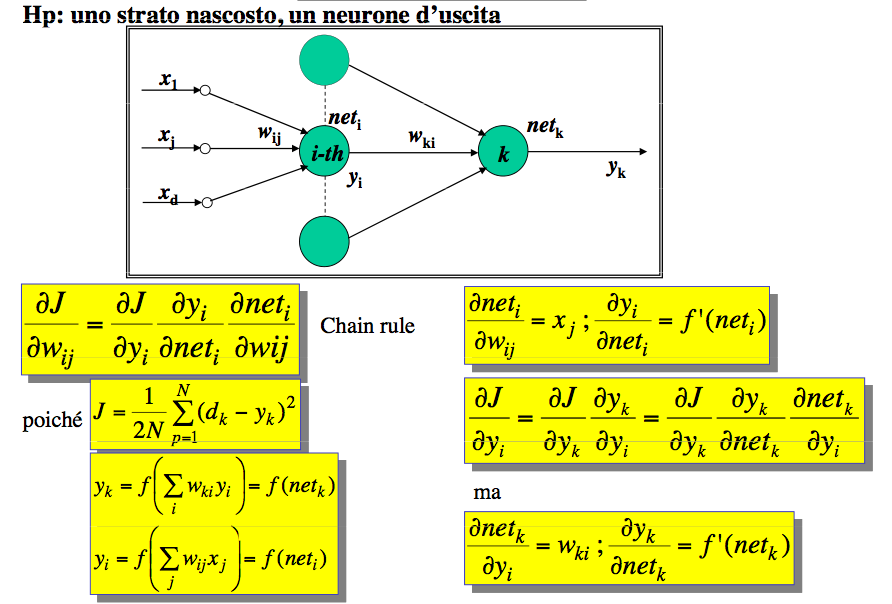
\includegraphics[scale=0.5]{img/hp.png}
\caption{}
\label{hp1}
\end{figure}
$J$ è una funzione di errore che dipende da $y_i$ e $y_i = f(net_i)$ dove $net_i$ è dipendente dalla sommatoria di $w_{ij}$. 
Poiché l'errore che misuriamo non è altro che la somma degli scarti al quadrato allora il valore calcolato da ogni neurone non è altro che una funzione $net_i$, quindi vengono calcolate le varie derivate: la derivata parziale di $net_i$ rispetto a $w_ij$ non è altro che $x_j$, la derivata di $y_i$ rispetto a $net_i$ non è altro che $f'(net_i)$. A questo punto sostituiamo ed abbiamo derivata di $J$ rispetto ad $y_i$, qui però abbiamo ciò che si differenzia dalla procedura precedente, la derivata la possiamo fare solo per $y_i$ che è di output perché soltanto per l'output è possibile calcolare la derivata parziale di $J$ rispetto ad $y_i$, adesso però vogliamo eseguire lo stesso procedimento ad un neurone che non è di output ma è un neurone hidden, quindi la derivata parziale di $J$ rispetto ad $y_i$ non la posso calcolare perché non abbiamo il target, cioè non ho il $d_i$ ma ho $d_k$, cioè il valore desiderato di output, quindi non ho il valore desiderato del neurone hidden. Quindi fin tutto è uguale  al procedimento di prima tranne per la derivata di $J$ rispetto a $y_i$. 
Allora facendo gli opportuni riarrangiamenti otteniamo quello mostrato in figura \ref{hp2} dove $e  = -(d_k - y_k)$.
\begin{figure}
\centering
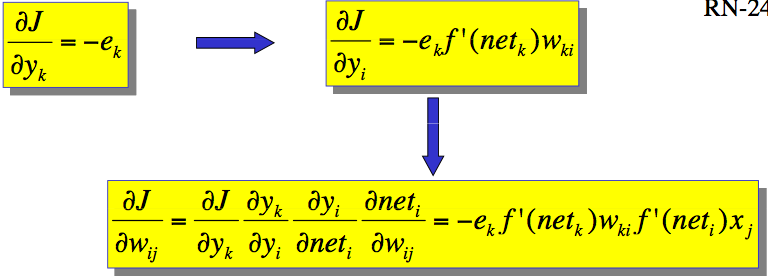
\includegraphics[scale=0.5]{img/hp2.png}
\caption{}
\label{hp2}
\end{figure}
\noindent Quindi abbiamo calcolato al derivata di $J$ rispetto a $w_{ij}$, che non è altro che l'incremento differenziale del gradiente. Ricordiamo che la regola è sempre la stessa
\begin{equation}
w(n+1) = w(n) - \eta \nabla J(w)
\end{equation}
il gradiente non è altro quello che abbiamo calcolato precedentemente
\begin{equation}
w_{ij}(n+1) = w_{ij}(n) - \eta \frac{\partial J}{\partial w_{ij}}
\end{equation}
e andando a sostituire otteniamo la regola di aggiornamento dei pesi per un neurone hidden 
\begin{equation}
w_{ij}(n+1) = w_{ij}(n) + \eta e_k(n) f'(net_k(n)) w_{ki}(n) f'(net_i(n)) x_j(n)
\end{equation}
Tutto questo ragionamento era soltanto per un neurone output, quando abbiamo $M$ neuroni di uscita il tutto si complica un pò (fig \ref{hp3}),
\begin{figure}
\centering
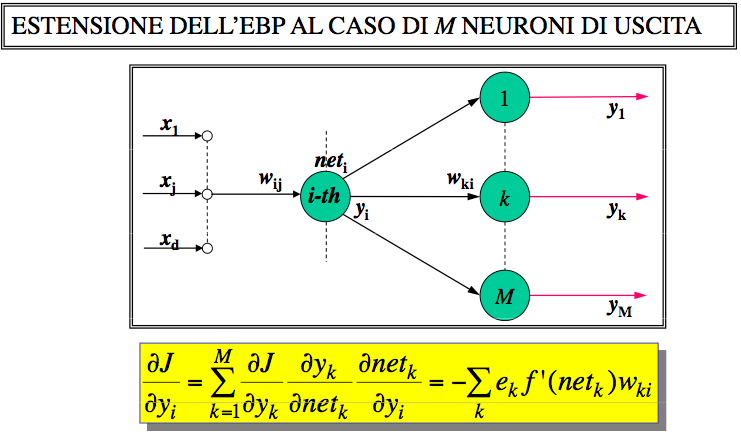
\includegraphics[scale=0.5]{img/hp3.png}
\caption{Più neuroni di output}
\label{hp3}
\end{figure}
perchè a questo punto al derivata di $J$ rispetto ad $y_i$ non è soltanto il prodotto tra gli elementi, ma è la sommatoria per $k$ che va da uno ad $M$, quindi a quello che abbiamo visto prima applichiamo soltanto la sommatoria, quindi andando a sostituire nella formula generale otteniamo
\begin{equation}
\frac{\partial J}{\partial w_{ij}} = - \left[ \sum_k e_k f'(net_k) w_{ki} \right] f'(net_i)x_j
\end{equation}
estendiamo ancora ed analizziamo il caso in cui abbiamo più strati nascosti (fig. \ref{hp4})
\begin{figure}
\centering
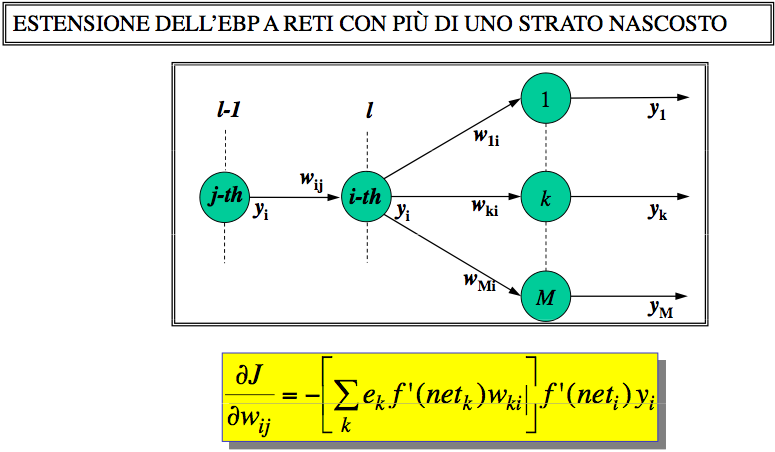
\includegraphics[scale=0.5]{img/hp4.png}
\caption{Più strati nascosti}
\label{hp4}
\end{figure}
la regola precedente si applica banalmente anche al caso di più strati nascosti perchè l'idea è a retropropagazione, cioè prima aggiorno i peso fra lo strato output e l'ultimo strato nascosto, poi a catena (retropropagazione) aggiorno i pesi tra il penultimo strato nascosto fino allo strato adiacente ai neuroni di input, quindi fondamentalmente la regola è la stessa soltanto che si applica a retropropagazione.\\

\noindent Riassumiamo il tutto definendo la regola finale
\begin{description}
\item[step 1 :] Presentare alla rete il pattern  $\{x_1, d_1\}$ 
\item[step 2 : Forward Step] La rete viene alimentata dal primo input poi vengono calcolati passo dopo passo (strato dopo strato) tutti i valori delle funzioni di attivazione, fino ad arrivare all'output, quindi indipendentemente da quanti neuroni nascosti e quanti strati nascosti ci sono bisogna arrivare all'output perché è l'unico punto dove si può calcolare l'errore. Dopo calcolato l'errore degli strati nascosti si passa allo step 3.
\item[step 3 :] clacoliamo l'errore dello strato di uscita
\item[step 4 : Backward Step] Quest'errore lo retropropaghiamo con la regola detta in precedenza in tutti i neuroni degli strati nascosti e applichiamo le regole di aggiornamento 
\item[step 5 :] Ripetere questa procedura per tutti i pattern del training e per il numero di epoche richiesto per la convergenza ( per evitare il problema che il percettrone apprendeva sempre l'ultimo pattern processato allora si randomizzano i pattern tra un’epoca e l’altra) e ripetere finché non si minimizza l'errore, quindi fintanto che l'errore $J$ non rientri sotto una determinata soglia.
\end{description}

\section{Learning non supervisionato}
Siamo nel caso in cui non conosciamo l'output desiderato. Il punto essenziale è noi non abbiamo più il target desiderato quindi non possiamo più misurare l'errore all'output e quindi non possiamo neanche retropropagare quest'errore dall'output allo strato hidden come è stato fatto nel caso supervisionato.  Parte del nostro cervello si rapporta proprio tra correlazione tra causa ed effetto (cioè: se faccio questo cosa succede?). Quindi per il funzionamento del cervello non c'è una regola propria che potrebbe essere tentata di codificare, ma ci deve essere qualche cosa che è ancora oscuro. La regola non è nota a priori ma è una regola che si adatta di volta in volta. Vediamo come è stato affrontato il problema da Hebb.\\

\subsection{Learning Hebbiano}
\noindent Nel 1940, Donald Hebb studiando la comunicazione tra neuroni, verificò che l’eccitazione ripetuta di un neurone $i$ da parte di un neurone $j$ portava all’abbassamento della soglia di eccitazione del neurone $i$ (FIg. \ref{hebb}).  Cioè se il neurone $i$ assumeva un valore molto alto della sua attivazione, quindi si eccitava molto rispetto al valore in entrante (valore del neurone a cui afferiva), dopo un po' di tempo andava in saturazione, quindi si abituava a questa forma di eccitazione e di conseguenza non rispondeva più alla stessa maniera di prima con il risultato che si abbassava la soglia di eccitazione del neurone $i$. 
\begin{figure}[h]
\centering
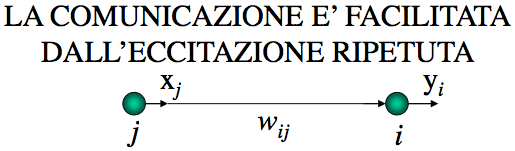
\includegraphics[scale=0.5]{img/hebb.png}
\caption{}
\label{hebb}
\end{figure}
Quindi fondamentalmente la comunicazione è facilitata dall'eccitazione ripetuta. Prima bisogna misurare qual'è l'eccitazione, poi bisogna vedere qual'è la causa $x_i$ e l'effetto $y_i$, ciò che lega causa ed effetto è proprio $w_{ij}$, ma la cosa più importante è la ripetizione, quindi prevale un aspetto di tipo statistico, più volte capita questo evento più il risultato è positivo. Infatti la regola di Hebb dice proprio che Il peso $w_{ij}$ della connessione tra i neuroni $i$ e $j$ cresce al fluire di un segnale da $j$ a $i$. Questa regola è nata da studi su scimmie e ratti e quindi si misurava esattamente il livello di eccitazione tra il segnale prodotto da un neurone in virtù dei neuroni afferenti ad esso e i neurotrasmettitori crescevano di entità che è proprio il peso della connessione $w_{ij}$. 
\begin{equation}
\nabla w_{ij} = \eta \cdot x_j y_i
\end{equation}
Quindi $w_{ij}$ aumenta al fluire di un segnale da $j$ ad $i$, fondamentalmente più fluisce in modo ripetuto questo segnale più $w_{ij}$ cresce. Quindi l'incremento è direttamente proporzionale al prodotto (o meglio la correlazione) tra $x_j$ ed $y_i$. La regola di quindi di aggiornamento prende la seguente forma
\begin{equation}
w(n+1) = w(n) +  \eta \cdot x_j y_i
\end{equation}
è molto diverso dalla regola vista precedentemente, perchè la vecchia misura molto l'errore commesso tra il valore prodotto ed il valore desiderato. In questo caso è indipendente dal valore target, quindi non supervisionato.\\
\noindent 
Possiamo vedere la correlazione tra i due valori in modo esteso affrontando il caso in cui abbiamo più input ed un solo output (fig. \ref{fig1}), dove l'output è per esempio un output lineare (quindi come combinazione lineare), allora $y$ può essere visto come
\begin{equation}
y= \sum_{i=1}^D w_i \cdot x_i = w^T \cdot x = x^T \cdot w = \abs{w} \cdot \abs{x} \cdot \cos \theta
\end{equation}

\begin{figure}
\centering
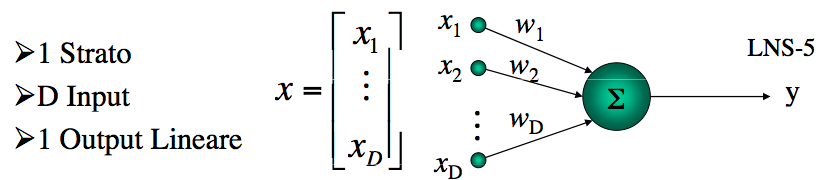
\includegraphics[scale=0.5]{img/fig1.png}
\caption{Caso non supervisionato: più input ed un solo output}
\label{fig1}
\end{figure}

quindi $y$ diventa grande quando $\theta$ diventa piccolo (cioè quando i due diventano molto più simili possibili), assumendo questo ci accorgiamo che l'ampiezza di $y$ misura la somiglianza tra il vettore di input ed il vettore dei pesi, quindi non misuriamo la distanza che intercorre tra il valore output del neurone  e il valore desiderato, ma il confronto lo facciamo tra l'input ed il vettore dei pesi. Quindi i pesi sono la memoria a lungo termine della rete, cioè alla fine ma mano che $y$ diventa sempre maggiore allora vuol dire che stiamo apprendendo i pattern in input. Fondamentalmente c'è una codifica non quantificabile ma è nei pesi e questo porta al termine che tipicamente viene attribuito alle reti neurali ovvero \emph{sistema distributivo di connessioni}, la rete neurale è un sistema altamente parallelo, ogni neurone può calcolare la sua funzione di attivazione indipendentemente dall'altro, dipende soltanto dai pesi della connessione, di conseguenza è assolutamente distribuito ed è altamente parallelo, quindi gli studi di questo sono anche di tipo ingegneristico, infatti Federico Faggin è stato il primo a progettare un mocrochip che si basava sulle reti neurali. L'idea era quella di realizzare una macchina basata sulle reti neurali, che è una logica diversa da quella che si basano le macchine in quanto sono operazione di algebra booleana.\\

\noindent La regola di aggiornamento dice
\begin{equation}
w_{new} = w_{old} +  \eta \cdot x_j y_i
\end{equation}
è possibile riscrivere come 
\begin{equation}
w_{new} = w_{old} +  \eta \cdot x \cdot w_{old} x
\end{equation}
perchè $y$ se è un unico neurone calcola il valore di $x$ per il peso quindi posso scrivere $y=w x$, metto in evidenza ed ottengo
\begin{equation}
w_{new} = w_{old}(1 + \eta \cdot x^2) 
\end{equation}
ma c'è un problema, vediamo che il $w_{new}$ è uguale al $w_{old}$ moltiplicato di una quantità positiva, che è talmente positiva che è il quadrato dell'input, quindi questo peso nuovo tende a crescere all'infinito.

\subsection{Regola di Oja}
Questo non va bene e quindi Oja stabilizza la regola, si pone il problema di non far tendere $w$ all'infinito,  vincola la crescita dei pesi che è possibile fare in due metodi:
\begin{itemize}
\item normalizzazione dei pesi dopo l'aggiornamento: 
\begin{equation}
w_i' = \alpha \cdot w_i \quad \quad \quad \quad \abs{w'} = 1
\end{equation}
però questo non è molto efficace come risultato, immaginiamo che in una rete neurale bisogna normalizzare tutti questi pesi, per normalizzare perdo una delle caratteristiche peculiari della rete stessa, il fatto che è altamente parallela. 
\item Aggiungere un termine proporzionale a $y^2$, nella formula di Hebb, quindi l'incremento è uguale a
\begin{equation}
\nabla w =\eta \cdot y \cdot (x  - y \cdot w)
\end{equation}
è uguale a quella vista in precedenza infatti sviluppando si ottiene proprio la regola di oja, cioè un freno alla crescita elevata del peso.
\end{itemize}

\noindent Hebb ha tanti vantaggi ed uno è la regola di aggiornamento on-line (quindi passo dopo passo), in questo caso abbiamo
\begin{equation}
\nabla w(n)= \eta\cdot y(n) \cdot x(n)= \eta \cdot x(n) \cdot x(n)^T \cdot w(n)
\end{equation}
se invece facciamo l'aggiornamento in bach, quindi l'aggiornamento viene effettuato dopo che il sistema ha visionato tutti i pattern allora la regola diventa
\begin{equation}
\nabla n = \eta \cdot \left( \sum_{i=1}^N x(i) \cdot x(i)^T \right) \cdot w(0) = \eta \cdot \hat{R}_x \cdot w(0)
\end{equation}
dove $\hat{R}_x$ è la matrice di correlazione del dataset.  Il vantaggio principale è che la matrice di autocorrelazione si può calcolare in modo poco costoso nel caso di apprendimento on-line ed in modo costoso nel caso off-line.\\
\noindent Riprendiamo la regola di oja che come abbiamo visto è
\begin{equation}
\nabla w_i = \eta  \ y(x - y w_i)
\end{equation}
quindi il problema di mantenere i pesi in norma unitaria viene risolto utilizzando il freno $-y w_i$. Se la analizziamo con attenzione ci accorgiamo che 
\begin{equation}
w_i(n+1) = \frac{w_i(n) + \eta \ y(n) \ x(n)}{\left[ \sum_{i=1}^D (w_i(n) + \eta \ y(n) \ x(n))^2 \right]^{1/2}}
\end{equation}
non facciamo altro che normalizzare i pesi, infatti al numeratore abbiamo la regola Hebbiana, quindi il peso nuovo è uguale al peso vecchio più $\eta$ moltiplicato il valore del neurone di output e il valore dell'input fratto la sommatoria di tutti gli incrementi (in quanto per normalizzare dobbiamo divide per la sommatoria di tutti gli altri pesi), se sviluppiamo per $\eta$ piccolo ci accorgiamo che questo può essere visto approssimativamente come   
\begin{equation}
w_i(n) + \eta \ y(n) [ x_i(n) - y(n) w_i(n) ] + O(\eta^2)
\end{equation}
è stata fatta l'espansione in serie di Taylor (che non viene dimostrata) di una funzione normalizzata di valori di peso. Oja prima ha preso la regola di Hebb, poi dopo l'aggiornamento normalizza i pesi in modo tale che la norma sia uguale ad uno, a quel punto sviluppa in serie di Taylor la funzione e ottiene la formula che è la regola di Oja. Posto
\begin{equation}
x_i'(n) = x_i(n) - y(n) w_i(n)
\end{equation}
allora
\begin{equation}
w_i(n+1) = w_i(n) + \eta \ y(n) \ x_i'(n)
\end{equation}
quindi la regola di Oja non fa altro che normalizzare i vettori dei pesi.\\

\noindent Adesso vediamo un altra particolarità della regola di Oja. Ipotizziamo di avere i pattern in uno spazio bidimensionale $x = [x_1, x_2]$, quando andiamo a calcolare $w$, secondo la regola di Oja i pesi dovrebbero disporsi quanto più prossimi alla disposizione dei pattern, quindi la similarità del peso e dei pattern deve essere la stessa, ora i pattern sono uguali, quindi qual'è il vettore $w$ che più si approssima a vettori dei dati? Quello che si trova sulla direzione principale dell'ellisse che circonda questi pattern (fig \ref{pattern}), 
\begin{figure}
\centering
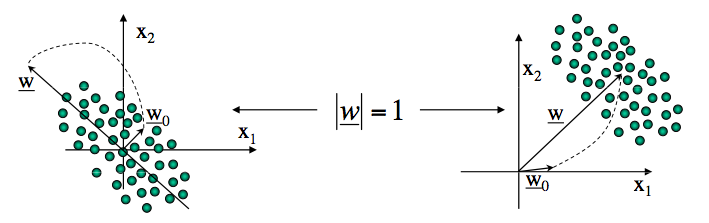
\includegraphics[scale=0.5]{img/pattern.png}
\caption{Esempio}
\label{pattern}
\end{figure}
quindi quelli a massima varianza, ci aspettiamo che dopo l'apprendimento Hebbiano il $w$ sia più simile a tutti i quanti i pattern se si dispone lungo l'asse principale dell'ellisse che circonda i pattern. Ma la direzione principale di questa ellisse non è quella per cui i dati si sono disposti con massima varianza? Come possiamo osservare per l'asse secondario la varianza è più piccola di quella che invece c'è sull'asse principale, quindi il $w$ ha una lunghezza che è proporzionale alla massima varianza, quindi fondamentalmente quello che stiamo dicendo è che la regola di Oja serve per determinare le componenti principali, quindi analizza i dati e i $w$ si dispongono esattamente sulle componenti principali (quindi sugl'assi principali del dataset) e quindi gli output della rete neurale con regola di aggiornamento di Oja non sono altro che le componenti principali del dataset.

\section{Reti Competitive e di Kohonen}
Anche in questo caso affrontiamo un problema di tipo non supervisionato. L'apprendimento competitivo nasce da un idea neurofisiologica. Nel nostro cervello ci sono delle mappe, ci sono aree che rispondono in modo massimale a certe attività sensoriali piuttosto che ad altre, per cui se guardiamo il cervello umano nella sua schematizzazione possiamo suddividerlo in aree: ci sono aree che si occupano dell'attività motoria, altre di attività uditive, altre di attività olfattorie, etc etc etc ...  Ci sono ovviamente interrelazioni fra le varie mappe ma è dimostrato che queste mappe possono anche non essere correlate al resto. Alcuni neuroni si specializzano ad alcune attività sensoriali, quindi si specializzano a certi gruppi di pattern di input piuttosto che ad altri. Nel modellare una rete neurale dobbiamo far si che un neurone o più neuroni possono rispondere in modo massimale, fondamentalmente danno una risposta della funzione di attivazione maggiore di tutti quante le altre se vengono forniti in ingresso alcuni input piuttosto che altri. Un problema è che non sempre i pattern sono disgiunti tra un attività sensoriale ed un altra per cui non sempre risponde quello che dovrebbe rispondere. In Fig \ref{mappa} che appare abbastanza disgiunta, infatti vediamo un neurone che si attiva in modo disgiunto rispetto agli altri, crea poche gerarchie (collaborazioni) con altri neuroni.
\begin{figure}
\centering
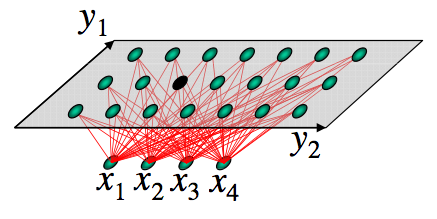
\includegraphics[scale=0.5]{img/rete.png}
\caption{Feature Mapping (Kohonen)}
\label{mappa}
\end{figure}
Quando vince un sol neurone stiamo parlando di apprendimento competitivo generico, un algoritmo in particolare che ha ottenuto maggiori riconoscimenti è quello dovuto a Kohonen ed è chiamato Self-Organizing Map,  il nome deriva dall'auto-organizzazione e dal mapping delle caratteristiche. L'idea è abbastanza semplice, si vuole riuscire a raggruppare i dati e quindi trovare mappe di neuroni che rispondo in modo massimale rispetto a gruppi di pattern soltanto con un solo strato (fig. \ref{mappe1}).
\begin{figure}
\centering
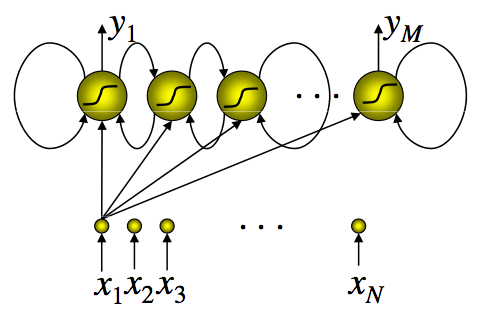
\includegraphics[scale=0.5]{img/mappe1.png}
\caption{}
\label{mappe1}
\end{figure}
Gli input possono essere tanti quante sono le componenti del pattern di input, tutti i neuroni di input sono connessi a tutti i neuroni di un unico strato che è sempre bidimensionale, questo strato rappresenta la mappa e a gruppi simili di dati rispondono neuroni vicini. Quindi pattern simili fanno si che neuroni vicini rispondono in modo massimale, questa è la proprietà topologica delle SOM. \'E un vincolo abbastanza forte, non soltanto voglio che vinca un neurone ma possono vincere anche  più neuroni, l'importante è che quelli che vincono sono vicini topologicamente tra loro, laddove però i pattern sono simili, allora quindi da una misura di dissimilarità in uno spazio euclideo a $d$ dimensioni si sta introducendo una vicinanza topologica in uno spazio bidimensionale, questo equivale ad un associazione tra vettori in uno spazio a $d$ dimensioni in uno spazio bidimensionale modificando la vicinanza, cioè la similarietà diventa vicinanza in termini topologici. Come realizzare ciò era l'obiettivo di Kohonen.\\  

\noindent Vediamo prima l'algoritmo classico competitivo, abbiamo tanti neuroni di input quante sono le dimensioni del pattern in ingresso e tanti neuroni output quante sono le classi che vengono codificate mediante la tecnica one-leave-out. La funzione è logistica quindi tende asintoticamente a 1 o a -1, oppure a 0 o a 1 a seconda della funzione di attivazione. 
La funzione è una combinazione lineare tra le componenti dei pattern entranti per i pesi. Sia il vettore delle osservazioni
\begin{equation}
x = [x_1, \dots, x_N]
\end{equation}
ed i possibili output
\begin{equation}
y = [y_1, \dots, y_M]
\end{equation}
allora la funzione i cui parlavamo prima espressa come combinazione lineare è
\begin{equation}
h_i = \sum_j w_{ij} \cdot x_j = w_i^T \cdot x
\end{equation}
Per esempio se prendiamo tutti gli $x_1, \dots, x_N$ che sono collegati tutti ad $y_1$, allora $y_1$ è la sommatoria dei pesi degl' archi per i pattern entranti. $h_i$ (che nel caso supervisionato è il $net_i$) può essere scritto come prodotto interno di $w_i$ ed $x$, quindi il prodotto interno del vettore peso relativo al neurone $i$ per il pattern di ingresso $x$, fondamentalmente stiamo misurando la distanza che intercorre tra i due vettori che è direttamente proporzionale al prodotto dei moduli per il coseno dell'angolo compreso,  più piccolo è l'angolo più grande è la distanza e viceversa, ed è zero quando i due vettori sono perpendicolari. Tra tutti i neuroni, in base a questa distanza, c'è un vincitore, quello che assume il valore massimo rispetto a tutti quanti gli altri. In questo caso stiamo specializzando soltanto un neurone, $i^*$ rappresenta il vettore peso del neurone che vincitore
\begin{equation}
i^* : w_{i^*} \cdot x \geq w^T \cdot x
\end{equation}
a questo punto il valore della funzione di attivazione che attribuisco a quel neurone per cui ho la correlazione massima tra $w_i$ e $x$ è uno, tutti quanti gli altri sono 0 (eccito uno ed inibisco tutti quanti gli altri).  In sintesi abbiamo $M$ vettori peso di lunghezza $N$, per un totale di $N \times M$ pesi,  il vettore peso ha la stessa dimensione dell'input ed è quel vettore che devo andare a confrontare con l'input, quanto più prossimo è $w$ ad $x$ (quindi l'angolo è piccolo) allora ho massima correlazione, quindi sono vicini. Ovviamente di volta in volta bisogna aggiornare i pesi. Questa è la rete competitiva classi classica e viene chiamata WTA (winner take all). \\

\noindent All'inizio i vettori peso sono tutti casuali poi devono essere aggiorniamo, immaginiamo di avere $p$ pattern $x_1, \dots, x_p$ e di volerli raggruppare, alcuni di questi devono far si che un unico neurone risponda in modo massimale e gli altri zero, per fare in modo che la risposta sia massimale allora devo fa si che la differenza tra $x$ e $w$ sia la più piccola possibile. Osservando la figura \ref{learn},
\begin{figure}
\centering
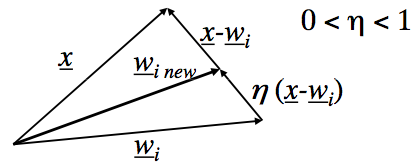
\includegraphics[scale=0.6]{img/learn.png}
\caption{}
\label{learn}
\end{figure}
misuro la distanza tra $x$ e $w_i$ e poi devo calcolare un nuovo $w_i$ che è più vicino ad $x$, ma $w_{i \ new}$ è più vicino ad $x$ se praticamente è direttamente proporzionale alla differenza che intercorre tra $x$ e $w_i$, che è quel vettore tra $x$ e $w_i$. quindi $w_{i \ new}$ sarà sicuramente direttamente proporzionale ad $x-w_i$ che è la differenza di una percentuale che ce la da $\eta$ che è un valore compreso tra 0 ed 1 e ci da esattamente la percentuale di quello che adiamo a moltiplicare. Quindi
\begin{equation}
\Delta w_{ij} = \eta \cdot y_i (x_j-w_{ij}) 
\end{equation}
moltiplicato per $y_i$ perchè vogliamo che un $y_i$ assume valore 1, mentre gli altri assumono valore 0, cioè aggiorniamo soltanto quello che vince. Questa regola prende il nome di Regola Instar. Questo è l' apprendimento competitivo, dove però vince un solo neurone alla volta, non c'è mappa ma c'è soltanto uno strato di neuroni di output dove uno vince e gli altri perdono, quello che vince è la classe di appartenenza del pattern in ingresso. Sostanzialmente è un algoritmo di clustering, ma a differenza delle tecniche viste precedentemente non c'è nessuna motivazione di tipo probabilistico, ma si basa fondamentalmente su una emulazione dei comportamento celebrale. Questa tecnica è caratterizzata dai centroidi dei cluster, quindi alla fine non vengono trattati tutti i dati ma soltanto i centroidi, cioè quei punti che rappresentano il cluster. In questo caso i prototipi sono gli $M$ vettori peso $w_i$.\\

\noindent Queste reti sono caratterizzate dallo strato di input, da un solo strato di neuroni e vince soltanto un neurone. Immaginiamo di avere $p$ pattern e per qualche strano motivo questi $p$ pattern fanno vincere sempre lo stesso neurone, fondamentalmente è come se avessi messo $M$ neuroni ma soltanto uno mi risponde in modo massimale. \'E possibile ma non è ammissibile questa riposta, allora si introduce un fattore di aging, quindi quando vince sempre un neurone, dopo un certo numero di volte che vince invece di andare a prendere il primo valore massimo vado a prendere il secondo valore massimo, a patto che la distanza che intercorre tra il primo massimo ed il secondo massimo sia sufficientemente piccola. Questo modo di agire si chiama coscienza, dato che stiamo emulando i comportamento del cervello umano allora dobbiamo dare una giustificazione a questo fattore di aging, quindi viene vista come coscienza del neurone che dopo aver risposto un determinato numero di volte con valore massimo allora si inibisce lasciando spazio agli altri neuroni.\\

\noindent . Supponiamo di prendere due pattern $x_1, x_2$, ci aspettiamo che quando un pattern viene presentato in ingresso allora risponda in modo massimale un neurone piuttosto che l'altro, il fatto che risponde in modo massimale soltanto un neurone è una decisione troppo hard, dobbiamo introdurre una decisione un pò soft introducendo l'incertezza o gradi di appartenenza di un pattern ad un cluster.  Allora vogliamo che non risponda in modo massimale soltanto uno ma li prendiamo in considerazione tutti e realizziamo la mappa tale che i pattern che sono vicini nello spazio delle caratteristiche alla fine generano risposte dei neuroni topologicamente vicini nello strato preso in considerazione.  
In questo caso la rete è bidimensionale (fig. \ref{retebd}), i neuroni sono connessi tutti ai neuroni di input e sono connessi anche fra di loro.
\begin{figure}
\centering
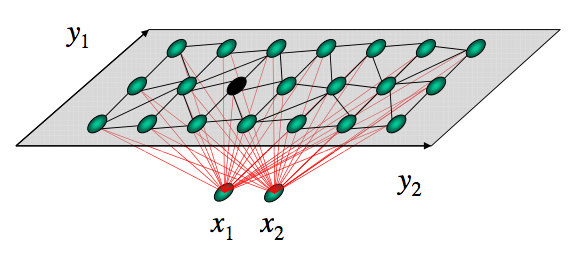
\includegraphics[scale=0.5]{img/retebd.png}
\caption{}
\label{retebd}
\end{figure}
Le connessioni nere rappresentano quelle tra neuroni allo stesso strato mentre le rosse rappresentano le connessioni tra i neuroni di output ed i neuroni di input.  Questo è il modello della rete neurale. Adesso si procede come prima, dato $x$ in ingresso, misuro la distanza che intercorre tra $x$ ed ogni vettore peso, calcoliamo il valore massimo ed otteniamo il neurone vincitore. L'unica differenza adesso è che non attribuiamo il valore uno al neurone vincitore e zero a tutti gli altri, non aggiorniamo soltanto il vincitore, ma vogliamo aggiornarli tutti, in particolare ci rifacciamo al fatto che ogni neurone risponde in modo massimale per i neuroni che si trovano nel vicinato del neurone vincitore in modo inibitorio man mano che ci si allontana, cioè la risposta è esattamente un cappello messicano (fig \ref{cappello}), dove nel centro di simmetria abbiamo il neurone vincitore, man mano che ci allontaniamo dal neurone vincitore gli altri rispondono anche loro in modo alto, ma in modo degradato, quindi fondamentalmente in modo submassimale rispetto al neurone vincitore, sia da un lato che dall'altro. 
\begin{figure}
\centering
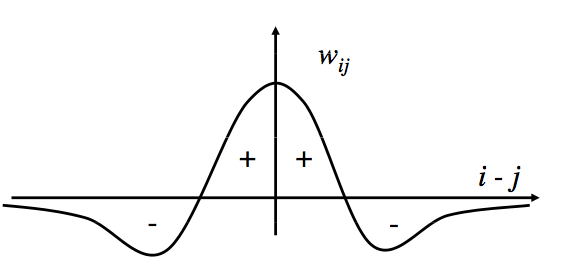
\includegraphics[scale=0.5]{img/cappello.png}
\caption{}
\label{cappello}
\end{figure}
Quando però siamo arrivati ai punti di massima varianza possibile, non è consentito che un neurone assuma un valore ancora ricettivo allo stimolo presentato, allora accade che inibisce, quindi saranno inibitori rispetto al quel neurone ma saranno eccitatori rispetto ad altri stimoli.\\

\noindent L'obiettivo è aggiornare tutti i pesi utilizzando la funzione che abbiamo visto, l'aggiornamento $\Delta w_{ij}$ lo facciamo per tutti i pesi, ma l'aggiornamento massimo si ha per il vincitore, poi man mano questo aggiornamento decresce secondo la curva gaussiana, in berve decersce mentre ci si allontana dal vincitore ed ad un certo punto diventa addirittura inibitorio. A questo punto introduciamo una funzione $\Lambda(i, i^*)$ che è funzione della distanza che intercorre tra un neurone nella posizione $i$ e il neurone nella posizione $i^*$ che è quello vincitore. Facendo così, tutti i pattern che sono vicini faranno si che i vincitori saranno vicini topologicamente nella mappa e quindi è possibile creare mappe per determinati stimoli. $\Lambda(i, i^*)$ è uguale ad uno per il vincitore $i^*$ (aggiorno in modo pieno il neurone vincitore). Gli altri invece li aggiorno secondo una funzione che è direttamente proporzionale alla distanza della posizione. L'unica cosa da definire è la funzione di vicinato, cioè l'intorno. Allora può essere sicuramente un otto intorno la cosa più semplice, oppure anche con un raggio maggiore, può essere esagonale, etc, etc, però c'è da considerare che qualsiasi forma di intorno che noi introduciamo, introduce una complessità nell'aggiornamento, quindi poco efficace.\\ 

\noindent La funzione radiale che abbiamo visto prima come cappello messicano è
\begin{equation}
\Lambda(i,i^*) = e^{- \abs{r_i - r_{i^*}}^2 / 2\sigma^2}
\end{equation}
All'inizio l'intorno viene scelto grande, poi man mano che aumentano le iterazioni questo intorno si riduce in modo tale che al limite diventa la rete competitiva iniziale, cioè quella che vince un sole neurone, oppure pochi neuroni, per cui quest'intorno diminuisce di raggio man mano che le iterazioni aumentano e per fare questo bisogna ridurre la varianza del cappello messicano, una regola è quella di applicare il $\sigma$  al passo $n$ come
\begin{equation}
\sigma(n) = \sigma_0 \left( 1 - \frac{n}{N_0} \right)
\end{equation}
ove $\sigma_0$ è la varianza iniziale, mentre $N_0$ è il numero massimo di iterazioni.  \\

\noindent Quanti neuroni output sono necessari per creare una mappa? i neuroni sono molto di più del numero di cluster poiché si deve creare l'aria che corrisponde ad un solo cluster. Non abbiamo più il centroide come nell'apprendimento competitivo, ma abbiamo un insieme di neuroni che rispondono in modo massimale. In conclusione abbiamo una clusterizzazione ma non abbiamo un identificazione precisa del centroide del cluster, ma ho più punti rappresentativi del cluster che sono i vettori peso dei neuroni che rispondono in modo massimale.\\

\noindent In seguto Kohonen ha realizzato una versione supervisionata di questo modello. Se invece si ha un solo neurone per ogni cluster, che equivale a dire il centroide del cluster (questa variante è chiamata LVQ (Learning Vector Quantization)) l'apprendimento emula il comportamento celebrale, però abbiamo un vantaggio che è la quantizzazione vettoriale, fondamentalmente stiamo quantizzando o discretizzando gruppi di vettori, e sto prendendo i rappresentativi per gruppi... (tutti i cluster sono quantizzazioni vettoriali). Anche questo è quantizzazione vettoriale nel caso ho pochi (o uno) neuroni per ogni cluster e nel caso in cui indichiamo chi deve vincere, non è che aggiorno in base a quello che vince, ma forzo a far vincere quel neurone in particolare. 

%
